%enemies.tex
Here a list of all enemies with a short description is given. Enemies information are obtained from: 
\begin{itemize}
	\item X1: \cite{wayback:X_resources},\cite{wiki:X1_enemies},
	\item X2: \cite{wayback:X2_resources},
\end{itemize}
while all artworks come from \cite{book:MMX_Complete_art}.

\section{Mini-Bosses}
\begin{itemize}
	\item \hypertarget{miniboss:Anglerge}{\textbf{Anglerge}}:
	\enemSpecs{64 (0.15 seconds of Iframe, Boomerang Cutter, Sting Chameleon and Rolling Shields hit for 8 damage) }{4 (contact), 2(snakes)}{Anglerge are angler-type mechaniloids that work to cleaning the seabed floor, with a motion sensor attached to its "lantern" part. Anglerge's attack are only four: send four snake-like robots toward X (two upward and two downward), which travel horizontally and descend when above (or below) X; a vacuum attack to push or pull X toward a spike pit; a (rare) energy beam from the angler (which can be disabled if the lamp is broken via an attack).}
	\begin{figure}[htp]
		\centering
		
\includegraphics[width=0.4\linewidth]{figures/X1/Enemies/Anglerge.jpg}
		\caption{Anglerge's artwork}
	\end{figure}
	
	\item \hypertarget{miniboss:Bee_Blader}{\textbf{Bee Blader}}:
	\enemSpecs{32 (No Iframes)}{4 (contact), 2(missiles), 1 (machine gun)}{A large bee-type helicopter which was created in order to carry \hyperlink{enem:Ball_De_Voux}{Ball de Voux}. It is equipped with a vulcan machine-gun and homing missiles. This mechaniloid has been created for guerrilla operations in forests and cities. While they don't appear formidable enemies, they can be rather dangerous, especially if X defeats them while standing below, as they will fall and crush him instantly.}
	\begin{figure}[htp]
		\centering
		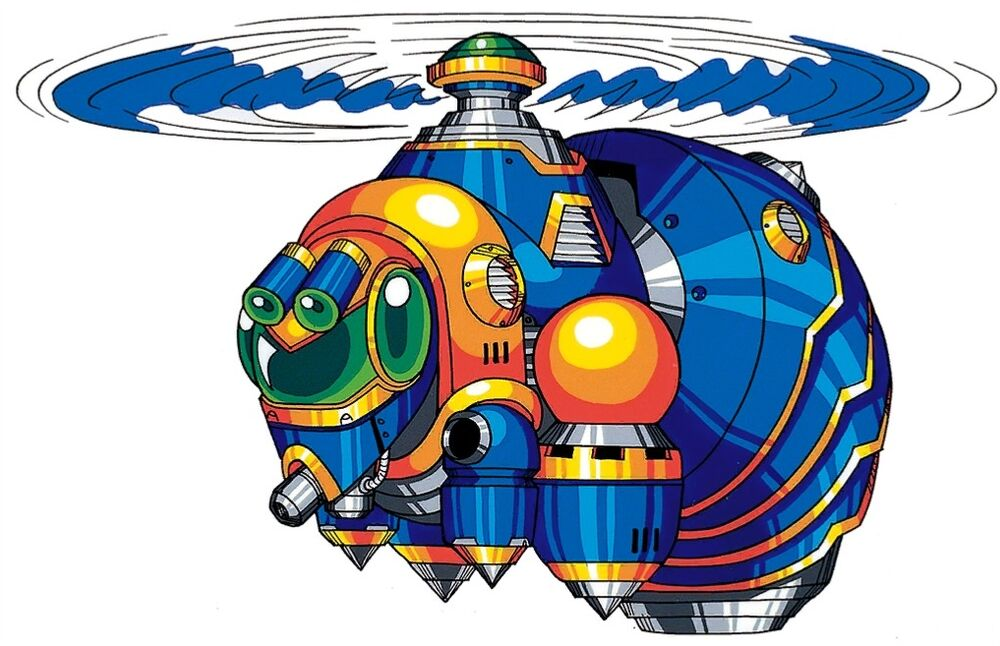
\includegraphics[width=0.5\linewidth]{figures/X1/Enemies/BeeBlader.jpg}
		\caption{Bee Blader's artwork}
	\end{figure}
	
	\item \hypertarget{miniboss:Chop_Register}{\textbf{Chop Register}}
	
	\item \hypertarget{miniboss:Cruiziler}{\textbf{Cruiziler}}: 
	\enemSpecs{64 (resist most weapons but no Iframes, meaning a Storm Tornado is a guaranteed kill)}{3 (bombs)}{Whale mechaniloid who patrols the sea with its powerful weapon. Some kind of mistake caused it to lose its sea navigation, its attack circuits began running wild, and communications were lost. Its body is totally invincible, save for its core on top.}
	\begin{figure}[htp]
		\centering
		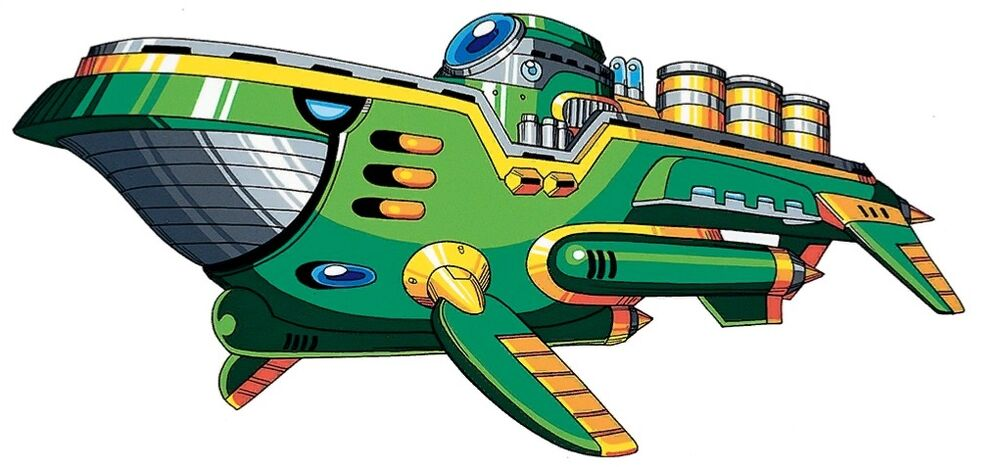
\includegraphics[width=0.4\linewidth]{figures/X1/Enemies/Cruiziller.jpg}
		\caption{Cruiziller's artwork}
	\end{figure}
	
	\item \hypertarget{miniboss:Magna_Quartz}{\textbf{Magna Quartz}}
	
	
	\begin{figure}[htp]
		\centering
		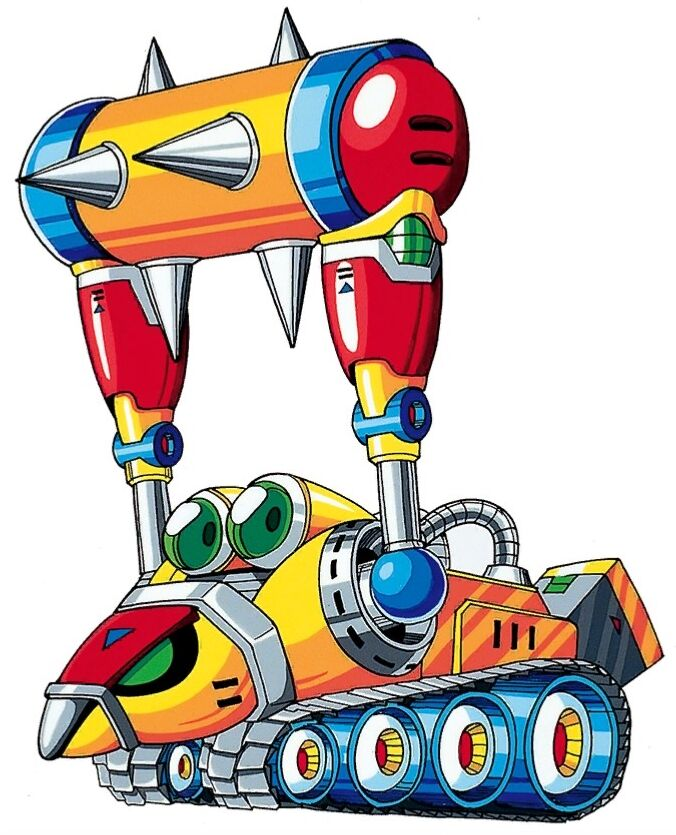
\includegraphics[width=0.3\linewidth]{figures/X1/Enemies/MoleBorer.jpg}
		\caption{Mole Borer's artwork}
	\end{figure}
	
	\item \hypertarget{miniboss:Mole_Borer}{\textbf{Mole Borer}}:
	\enemSpecs{60 ($\sim$0.083 seconds of Iframes. Fire Wave deals 3 damage each 2 frames)}{Insta-kill (roller), 2 (contact)}{Mechanioid used to open up paths in mines, using a rotary roller to destroy rocks that obstruct his path. Its armoring can take a lot of damage, while the roller is completely invincible and can instantly kill X. The only way to deal with it is to attack from behind, although several shots are needed to take it down. Using the Fire Wave is the best option, as its continuous damage can dispose of it quickly.}
	
	\item \hypertarget{miniboss:Old_robot}{\textbf{Old Robot}}
	
	\item \hypertarget{miniboss:Paraloid_S-38}{\textbf{Paraloid S-38}} 
	
	\item \hypertarget{miniboss:Raider_Killer}{\textbf{Raider Killer}}
	
	\item \hypertarget{miniboss:RT-55J}{\textbf{RT-55J}}: 
	\enemSpecs{64 (0.5 second of Iframes, resist most weapons. Boomerang Cutter deals 3 damage instead of 2)}{2 (contact), 2 (arm)}{In times of peace, it was a professional robot sumo wrestler and a popular Yokozuna (sumo grand champion) in the "Robot Grand Sumo Tournament". Moved in the forest, it now guards X's  Chest Parts. Its certain kill technique, the "Kagizume Beam Hand," strikes and tosses its opponents but only if it is in his claw's reach range. Otherwise he'll just jump at it to close the gap.} 
	\begin{figure}[htp]
		\centering
		
\includegraphics[width=0.3\linewidth]{figures/X1/Enemies/RT-55J.jpg}
		\caption{RT-55J's artwork}
	\end{figure}
	
	\item \hypertarget{miniboss:Sea_Canthller}{\textbf{Sea Canthller}}
	
	\item \hypertarget{miniboss:Thunder_Slimer}{\textbf{Thunder Slimer}}: 
	\enemSpecs{48 (0.116 seconds of Iframes, Storm Tornado hits for 9-10 damage)}{5(contact), 4(thunders)}{Thunder Slimer was born from a single question: ``How large can a single cell become?'' This monster was born from said experiment. Its body is over three times as large as X, but may require approximately 10 years before it reaches full growth. It has settled in the power plant, where he absorbs electricity and uses it to perform electric attacks against X.}
	\begin{figure}[htp]
		\centering
		
\includegraphics[width=0.3\linewidth]{figures/X1/Enemies/ThunderSlimer.jpg}
		\caption{Thunder Slimer's artwork}
	\end{figure}
	
	\item \hypertarget{miniboss:Utuboros}{\textbf{Utuboros}}: 
	\enemSpecs{72 (no Iframes, Boomerang Cutter hits for 3 damage instead of 2 and Storm Tornado kill it in a single shot)}{4 (contact)}{Serpent-type mechaniloid made to explore the ocean floor. Thanks to its flexible body it can zig-zag into difficult underwater areas, and burrow underground. His body is totally invincible and can work as a platform, while only the head and tail are vulnerable and can damage X.}
	\begin{figure}[htp]
		\centering
		
\includegraphics[width=0.4\linewidth]{figures/X1/Enemies/Utuboros.jpg}
		\caption{Utuboros's artwork}
	\end{figure}
\end{itemize}



\section{Minor enemies}
\begin{itemize}
	\item \hypertarget{enem:Aclanda}{\textbf{Aclanda}}
	
	\item[{
\includegraphics{figures/X1/Enemies/sprite_amenhopper.png}}] \hypertarget{enem:Amenhopper}{\textbf{Amenhopper}}: 
	\enemSpecs{2}{1 (bombs), 2(contact)}{Originally designed for farm work, it was used to sow fertilizer 
		across the land. Now, it's been remodeled into a bomb-dropping
		battle type mechaniloid.}
	
	%	\begin{itemize}
	%		\item \textbf{HP}: 2
	%		\item \textbf{Damages}: 1 (bombs), 2(contact)
	%		\item \textbf{Description}:Originally designed for farm work, it was used to sow fertilizer 
	%		across the land. Now, it's been remodeled into a bomb-dropping
	%		battle type mechaniloid.
	%	\end{itemize}
	
	\item[ {
\includegraphics[height=20px]{figures/X1/Enemies/sprite_armor_soldier.png}}] \hypertarget{enem:Armor_Soldier}{\textbf{Armor Soldier}}: 
	\enemSpecs{3 (on foot), 16 (Ride Armor)}{2 (contact, on foot), 3(contact-Armor)}{Lowest class of soldier reploids, used in military affairs. Riding in their Ride Armor, they do destruction work under Sigma's orders.}
	
	\item[{
\includegraphics[width=30px]{figures/X1/Enemies/sprite_axemax.png}}] \hypertarget{enem:Axe_Max}{\textbf{Axe Max}}:
	\enemSpecs{8}{3 (contact, on foot), 2(flying log)}{Woodcutter reploid from the forest, remodeled for brutality. Swinging his large axe, he attacks by sending the chopped wood flying.}
	
	\item[{
\includegraphics[height=20px]{figures/X1/Enemies/sprite_balldevoux.png}}] \hypertarget{enem:Ball_De_Voux}{\textbf{Ball De Voux}}:
	\enemSpecs{2}{1 (contact)}{Equipped with 2 soft-treading feet, this mecha can move over any topography.
		Inside the sphere there is a camera and a sensor which can even see in the dark.}
	
	\item \hypertarget{enem:Bar_Waying}{\textbf{Bar Waying}}
	
	\item \hypertarget{enem:Barite_Lastar}{\textbf{Barite Lastar}}
	
	\item \hypertarget{enem:Barrier_Attacker}{\textbf{Barrier Attacker}}
	
	\item[{
\includegraphics{figures/X1/Enemies/sprite_battonbone.png}}] \hypertarget{enem:Batton_Bone}{\textbf{Batton Bone}}:
	\enemSpecs{1}{1 (contact)}{Bat mechaniloids with a taste for humans. They dwell in forests and caves.}
	
	\item \hypertarget{enem:Batton_Bone_type_G}{\textbf{Batton Bone type G}}
	
	\item[{
\includegraphics[height=15px]{figures/X1/Enemies/sprite_battonm501.png}}]  \hypertarget{enem:Batton_M-501}{\textbf{Batton M-501}}: 
	\enemSpecs{2}{1 (contact)}{Bat type mechaniloid which the \hyperlink{enem:Batton_Bone}{Batton Bone} series is based on. It is a very unusual mechaniloid, made over 30 years ago.}
	
	\item \hypertarget{enem:Beetron}{\textbf{Beetron}}
	
	\item \hypertarget{enem:Blecker}{\textbf{Blecker}}
	
	\item[{
\includegraphics{figures/X1/Enemies/sprite_bombeen.png}}]\hypertarget{enem:Bomb_Been}{\textbf{> Been}}:
	\enemSpecs{2}{2 (contact), 1 (bomb)}{Small bee-modeled helicopter used for land mines scattering. Able to infiltrate any area, it can set up land mines anywhere.}
	
	\item \hypertarget{enem:Cannon_Driver}{\textbf{Cannon Driver}}
	
	\item[{
\includegraphics[height=20px]{figures/X1/Enemies/sprite_cragman.png}}] \hypertarget{enem:Crag_Man} {\textbf{Crag Man}}:
	\enemSpecs{8}{2(contact),2(rock fall)}{Crag Men were made to clear rock debris during landslides. They work actively with the aerial mechaniloid \hyperlink{enem:Sky_Claw}{Sky Claw}.}
	
	\item \hypertarget{enem:Crash_Roader}{\textbf{Crash Roader}}
	
	
	\item[{
\includegraphics[height=10px]{figures/X1/Enemies/sprite_creeper.png}}] \hypertarget{enem:Creeper} {\textbf{Creeper}}:
	\enemSpecs{1}{1 (contact)}{An insect-type mechaniloid. It's unknown what it was made for.	It is pecked out from the insides of trees by the \hyperlink{enem:Mad_Pecker}{Mad Pecker}.}
	
	\item \hypertarget{enem:Croak_hopper}{\textbf{Croak Hopper}}
	
	\item[{
\includegraphics[height=20px]{figures/X1/Enemies/sprite_crusher.png}}] \hypertarget{enem:Crusher}{\textbf{Crusher}}:
	\enemSpecs{2}{4}{Construction mechaniloid used for knocking down buildings. It drops its steel-made weight to scrape down the highway.}
	
	\item[{
\includegraphics[height=20px]{figures/X1/Enemies/sprite_diglabour.png}}] \hypertarget{enem:Dig_Labour}{\textbf{Dig Labour}}: 
	\enemSpecs{4}{2(pickaxe), 3(contact)}{The greatest pickaxe worker in the world. He is a diligent reploid who works in the robot factory.}
	
	\item \hypertarget{enem:Disk_Boy_08}{\textbf{Disk Boy 08}}
	
	\item[{
\includegraphics[height=20px]{figures/X1/Enemies/sprite_dodgeblaster.png}}] \hypertarget{enem:Dodge_Blaster}{\textbf{Dodge Blaster}}: 
	\enemSpecs{3}{2 (contact), 2(shots)}{Latest model of mobile cannon with "self-defense function", which makes it possible to avoid energy attacks before they can even get near it.}
	
	\item \hypertarget {enem:Fishern}{\textbf{Fishern}}
	
	\item[{
\includegraphics[height=20px]{figures/X1/Enemies/sprite_flamer.png}}] \hypertarget{enem:Flamer}{\textbf{Flamer}}:
	\enemSpecs{6}{3 (contact), 2(fire)}{High-temperature blaze-blowing flamethrower machine. A remodeled airport fire extinguisher mechaniloid, turned into a weapon which tries to spread fires.}
	
	\item[{
\includegraphics[height=30px]{figures/X1/Enemies/sprite_flammingle.png}}] \hypertarget{enem:Flammingle}{\textbf{Flammingle}}:
	\enemSpecs{8, 4-saw}{3 (contact), 2(blade)}{Flamingo-type mechaniloid taken from the robot zoo. It attacks by spinning its head and releasing the saw.}
	
	\item \hypertarget{enem:Garakuta_Robot}{\textbf{Garakuta Robot}} 
	
	\item[{
\includegraphics[height=20px]{figures/X1/Enemies/sprite_gulpfer.png}}] \hypertarget{enem:Gulpfer}{\textbf{Gulpfer}}:
	\enemSpecs{10}{2 (contact), 2-32 (eating)}{Once the ornamental mascot mechaniloid of a seaside Chaya teahouse, it escaped and was converted for catching ocean fish. It was originally based on an old children's toy.}
	
	\item[{
\includegraphics[height=20px]{figures/X1/Enemies/sprite_gunvolt.png}}] \hypertarget{enem:Gun_Volt}{\textbf{Gun Volt}}:
	\enemSpecs{16}{3 (contact), 2(sparks), 2(missiles)}{Mechaniloid developed for military use. A tank made for terrestrial combat, it attacks with missiles and high voltage bullets.}
	
	\item \hypertarget{enem:Hanged_Reploid}{\textbf{Hanged Reploid}}
	
	\item[{
\includegraphics[height=20px]{figures/X1/Enemies/sprite_hoganmer.png}}] \hypertarget{enem:Hoganmer}{\textbf{Hoganmer}}:
	\enemSpecs{8}{3 (contact), 2(spike ball)}{Fighter in the future grappling show "Robot Coliseum." It blocks the attacks of enemies with its shield, and attacks	by swinging its iron ball and chain.}
	
	\item[{
\includegraphics[height=20px]{figures/X1/Enemies/sprite_hotarion.png}}] \hypertarget{enem:Hotarion}{\textbf{Hotarion}}:
	\enemSpecs{1}{2 (contact)}{A mechaniloid for nighttime patrol, it was made to save the firefly appearance from extinction. Shining, it flies through the sky.}
	
	\item \hypertarget{enem:Installer}{\textbf{Installer}}
	
	\item[{
\includegraphics[height=20px]{figures/X1/Enemies/sprite_jamminger.png}}] \hypertarget{enem:Jamminger}{\textbf{Jamminger}}:
	\enemSpecs{2}{1 (contact)}{Mechaniloid that attacks any enemies who enter a forbidden area. An odd robot who laughs after attacking.}
	
	\item \hypertarget{enem:Jelly_Seeker}{\textbf{Jelly Seeker}}
	
	\item[{
\includegraphics[height=20px]{figures/X1/Enemies/sprite_ladderyadder.png}}] \hypertarget{enem:Ladder_Yadder}{\textbf{Ladder Yadder}}:
	\enemSpecs{3}{2 (contact)}{Originally a mechaniloid supervisor of the forest regions. It would locate any poachers, and report the forest's temperature and humidity to the woodland protection center.}
	
	\item[{
\includegraphics[height=20px]{figures/X1/Enemies/sprite_liftcannon.png}}] \hypertarget{enem:Lift_Cannon}{\textbf{Lift Cannon}}:
	\enemSpecs{2}{3(contact), 2(shot)}{Rotary-type cannon attached to a tube-like stand. Originally, a fire-fighting robot for control towers and any other high places in the airport.}
	
	\item[{
\includegraphics[height=20px]{figures/X1/Enemies/sprite_madpecker.png}}] \hypertarget{enem:Mad_Pecker}{\textbf{Mad Pecker}}:
	\enemSpecs{6}{2 (contact)}{Woodpecker-type repliroid who chops trees in the forest. Tries to follow \hyperlink{enem:Planty_Iworms}{Planty}, without success.}
	
	\item \hypertarget{enem:Mecha-Arm}{\textbf{Mecha-Arm}}
	
	\item[{
\includegraphics[width=30px]{figures/X1/Enemies/sprite_megatortoise.png}}] \hypertarget{enem:Mega_Tortoise}{\textbf{Mega Tortoise}}:
	\enemSpecs{16}{4(contact),3 (bombs)}{A turtle-type mechaniloid originally meant for rescuing humans from maritime disasters. From its back, it now produces bombs in place of floating devices.}
	
	\item[{
\includegraphics{figures/X1/Enemies/sprite_metalwing.png}}] \hypertarget{enem:Metal_Wing}{\textbf{Metal Wing}}: 
	\enemSpecs{1}{3 (contact)}{A reconnaissance mechaniloid. When it spots dangers, it raises its flying speed in a great rush to get news to its master.}
	
	\item[{
\includegraphics{figures/X1/Enemies/sprite_mettalc15.png}}] \hypertarget{enem:Metall_C-15}{\textbf{Metall C-15}}: 
	\enemSpecs{2}{2 (contact), 1(bullet)}{Reploid who watches factories. From the former series that worked in factories, now they are advanced enough to be placed as chiefs.}
	
	\item \hypertarget{enem:Morgun}{\textbf{Morgun}}
	
	\item \hypertarget{enem:Pararoid_R-5}{\textbf{Pararoid R-5}}
	
	\item \hypertarget{enem:Pararoid_V-1}{\textbf{Pararoid V-1}}
	
	\item[{
\includegraphics{figures/X1/Enemies/sprite_planty.png}}] \hypertarget{enem:Planty_Iworms} {\textbf{Planty\&Iworms}}: 
	\enemSpecs{2 (Planty), 1 (Iworm)}{3 (contact-Planty), 1(contact-Iworm)}{Planty is from the Mettool family and watches over the forest. From its head, it can manufacture the earthworm-type, soil cultivation reploid, Iworm.}
	
	\item[{
\includegraphics{figures/X1/Enemies/sprite_raybit.png}}] \hypertarget{enem:Ray_Bit}{\textbf{Ray Bit}}: 
	\enemSpecs{2}{4 (contact), 3 (laser)}{Rabbit-type mechaniloid taken from the robot zoo. It skips and jumps, using the laser cannon in its ears to attack.}
	
	\item[{
\includegraphics[height=15px]{figures/X1/Enemies/sprite_raytrap.png}}] \hypertarget{enem:Ray_Trap}{\textbf{Ray Trap}}: 
	\enemSpecs{-}{-}{Mechaniloid devices which await the false steps of intruders.}
	
	\item \hypertarget{enem:Refleczer}{\textbf{Refleczer}}
	
	\item \hypertarget {enem:Rideroid G}{\textbf{Rideroid G}}	
	
	\item \hypertarget{enem:Rightod}{\textbf{Rightod}}
	
	\item[{
\includegraphics[width=30px]{figures/X1/Enemies/sprite_roadattacker.png}}] \hypertarget{enem:Road_Attackers}{\textbf{Road Attackers}}: 
	\enemSpecs{12(total), at 7/12 the pilot dies; at 3/12 the engine explodes}{2 (contact), 1 (shot)}{A destructive reploid gang of hot-rodders, riding for Sigma's rebellion. Large beam cannons have been attached to the bonnets of their sports cars.}
	
	\item \hypertarget{enem:Road_Riders}{\textbf{Road Riders}}
	
	\item[{
\includegraphics{figures/X1/Enemies/sprite_rollinggabyoall.png}}] \hypertarget{enem:Rolling_Gabyoall}{\textbf{Rolling Gabyoall}}: 
	\enemSpecs{1 (Immune to all but Rolling Shield)}{3 (contact)}{Intruder repulsion robot. It Appears to be a simple mechaniloid, but truthfully, it possesses the human-like mind of a reploid.}
	
	\item[{
\includegraphics{figures/X1/Enemies/sprite_rushroader.png}}] \hypertarget{enem:Rush_Roader}{\textbf{Rush Roader}}: 
	\enemSpecs{6}{2 (contact)}{Leaders of the robot gang of hot-rodders. To get revenge on the Maverick Hunters who once chased them down, they became Sigma's subordinate.}
	
	\item \hypertarget{enem:Sabottein}{\textbf{Sabottein}}
	
	\item \hypertarget{enem:Scrambler}{\textbf{Scrambler}}
	
	\item[{
\includegraphics[height=20px]{figures/X1/Enemies/sprite_scraprobo.png}}] \hypertarget{enem:Scrap_Robo}{\textbf{Scrap Robo}}:
	\enemSpecs{4}{3 (contact), 2(laser))}{A pathetic upper body of a robot, made to become a car driver. Although it passed part of the humans' expectations, without a driver's license, it has been turned into scrap.}
	
	\item \hypertarget{enem:Scriver}{\textbf{Scriver}}
	
	\item[{
\includegraphics[height=20px]{figures/X1/Enemies/sprite_seaattacker.png}}] \hypertarget{enem:Sea_Attacker}{\textbf{Sea Attacker}}:
	\enemSpecs{2}{2 (contact)}{Seahorse-type mechaniloid created as a novelty for humans' homes. Its body somersaults as it charges.}
	
	\item[{
\includegraphics{figures/X1/Enemies/sprite_sinefaller.png}}] \hypertarget{enem:Sine_Faller}{\textbf{Sine Faller}}:
	\enemSpecs{1}{2 (contact)}{Aerial mechaniloid made with the idea "Quality from quantity". It flies and turns, acting as a hindrance.}
	
	\item[{
\includegraphics[height=20px]{figures/X1/Enemies/sprite_skyclaw.png}}] \hypertarget{enem:Sky_Claw}{\textbf{Sky Claw}}:
	\enemSpecs{2}{2 (contact), 3(self-destruct)}{A robot who removes obstacles, originally designed for the ``Crane Game'' which was popular in Japan during the later half of the twentieth century.}
	
	\item \hypertarget{enem:Sky_farmer}{\textbf{Sky Farmer}}
	
	\item \hypertarget{enem:Slidame}{\textbf{Slidame}}
	
	\item[{
\includegraphics[width=30px]{figures/X1/Enemies/sprite_slidecannon.png}}] \hypertarget{enem:Slide_Cannon}{\textbf{Slide Cannon}}:
	\enemSpecs{3}{2 (contact), 2(shot)}{Defensive artillery, set up to attack aerial enemies. Designed after the German anti-aircraft cannons of the 1940s.}
	
	\item[{
\includegraphics[height=20px]{figures/X1/Enemies/sprite_snowshooter.png}}] \hypertarget{enem:Snow_Shooter}{\textbf{Snow Shooter}}: 
	\enemSpecs{4}{3 (contact), 2(snowball)}{Bad-natured mechaniloid who toss balls of white iron as if they were snowballs. They are Chill Penguin's guardians.}
	
	\item \hypertarget{enem:Sole_solar}{\textbf{Sole Solar}}
	
	\item[{
\includegraphics[height=20px]{figures/X1/Enemies/sprite_spiky.png}}] \hypertarget{enem:Spiky}{\textbf{Spiky}}: 
	\enemSpecs{2}{2 (contact)}{Monocycle which bears sharp spikes in its tire. Very dangerous, its main attack technique is to slide over and self-destruct.}
	
	\item \hypertarget {enem:Tiranos}{\textbf{Tiranos}}
	
	\item[{
\includegraphics{figures/X1/Enemies/sprite_tombot.png}}] \hypertarget{enem:Tombot}{\textbf{Tombot}}:
	\enemSpecs{1}{2 (contact)}{A dragonfly-type glider. When taking off, it cuts and releases the jet propulsion units. Then, slowly riding the wind, it flies through the sky.}
	
	\item \hypertarget {enem:Tubamail_Generator}{\textbf{Tubamail Generator}}
	\item \hypertarget {enem:Tubamail-S}{\textbf{Tubamail-S}}
	
	\item[{
\includegraphics[width=20px]{figures/X1/Enemies/sprite_turncannon.png}}] \hypertarget{enem:Turn_Cannon}{\textbf{Turn Cannon}}: 
	\enemSpecs{5}{}{Robot once designed as a sprinkler for domestic use, but was defective until the water was replaced with cannon shells.}
	
	\item \hypertarget{enem:Weather_crystal}{\textbf{Weather Crystal}}
	
	
	
\end{itemize}











